%%%%%%%%%%%%%%%%%%%%%%%%%%%%%%%%%%%%%%%%%%%%%%%%%%%
%
%  New template code for TAMU Theses and Dissertations starting Fall 2016.
%
%
%  Original Author: Sean Zachary Roberson
%  This version adapted for URS by Parasol lab.
%  Adapted from version 3.16.10, which was last updated on 9/29/2016.
%  URS adaptation last updated 1/9/2017.
%
%%%%%%%%%%%%%%%%%%%%%%%%%%%%%%%%%%%%%%%%%%%%%%%%%%%
%%%%%%%%%%%%%%%%%%%%%%%%%%%%%%%%%%%%%%%%%%%%%%%%%%%%%%%%%%%%%%%%%%%%%%%
%%%                           SECTION II
%%%%%%%%%%%%%%%%%%%%%%%%%%%%%%%%%%%%%%%%%%%%%%%%%%%%%%%%%%%%%%%%%%%%%%

\chapter{THE ALGORITHM}


\section{Introduction}

The core portion of the platform that hopes to allow reordering of aspects of the textbook can simply summed up as \textit{The Algorithm}. This underlying algorithm is independent of technology stack or implementation. It is simply a high level description and analysis of the proposed solution to the given problem.

With simply an understanding of the algorithm, the implementation should follow in a natural and simple manner.

\section{The Motivation for the Algorithm}

The algorithm has other items to consider outside simply just solving the given issue. As with most algorithms, there is a thought and focus on completing the desired task in an efficient and optimal manner. This means that if the algorithm is able to provide feedback but if it is done in an clunky manner, the algorithm is still considered a failure.

In addition to efficiency, correctness is another major point of focus. In this context, correctness relates to properly conveying the thoughts and concerns of the original author to the professor or institution trying to modify the ordering of a textbook. As a result of a particular action or modification by the consumer, there should never arise a situation where a suggestion or warning provided by the algorithm conflicts with the thoughts or viewpoints of the author of the textbook. These messages provided by the algorithm should be simply an extension of the original if not exactly the same as if the author was at the computer sitting with the user of the platform.

Correctness also relates to truly reordering the textbook as desired and specified by the one who modified the order of the textbook. After a change by the consumer, they should be able to clearly understand what type of change they are proposing, how this affects the textbook as a whole, how nearby sections or chapters may be affected and finally after committing these changes, the actual textbook should properly reflect these changes as desired by the consumer. 

\textit{traverse old and new textbooks
diff algorithm between two trees}

\textit{traverse old and new textbooks
diff algorithm between two trees}

\cite{bile}
\cite{tsur}
\cite{reactReconcile}

\section{The Design}

The design includes\dots

tree of unit (chapters/sections/pages) order -- 1a orig and 1b modified

tree of exercise order -- 2a orig and 2b modified

tree of unit interdependences 3

tree of exercises dependencies on units 4

flexiblility 

1. author creates original trees 1a, 2a, 3, 4

2. adopting institution or instructor specifies desired order of units 1b \newline
   program provides warnings of impermissible orders as this tree is created \newline
   adopting institution or instructor can override order
   
3. program automatically creates 2b \newline
   adopting institution or instructor previews exercise and can override order
   
4. actually reorder the files of the text and links between them

% \begin{figure}[ht]
% \centering
% 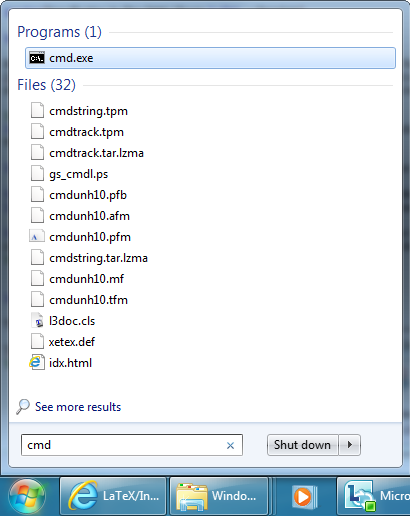
\includegraphics[scale=0.75]{TAMUthesis_CMD_windows.png}
% \caption[The command line compiler in Windows.]{The command line compiler in Windows. It is not suggested that you compile using this method. See compilation instructions in the README.}

% \label{fig:CMD_1}
% \end{figure}


% \begin{table}[h!]
% 	\centering
% 	\label{Band}
% 	\caption{Scores from the 2011 Arcadia Festival of Bands.}
%         \vspace{1em}
% 	\begin{tabular}{|l|l|l|}
% 		\hline
% 		School Name & Band Score & Auxiliary Score \\ \hline
% 		Rancho Bernardo & 96.15 & 89.15 \\ \hline
% 		Mt. Carmel & 95.30 & 83.55 \\ \hline
% 		Riverside King & 93.85 & 91.75 \\ \hline
% 		Diamond Bar & 93.20 & 88.60 \\ \hline
% 		El Dorado & 92.80 & 95.45 \\ \hline
% 		Chino & 92.65 & 91.45 \\ \hline
% 		Henry J. Kaiser & 92.60 & 87.55 \\ \hline
% 		Glendora & 92.60 & 89.15 \\ \hline
% 		Montebello & 90.50 & 82.70 \\ \hline
% 		Mira Mesa & 89.65 & 91.50 \\ \hline
% 	\end{tabular}
% \end{table}

% %Make other examples.
% \begin{equation} \label{Equ.2.1}
% y=c_1\cos(t)+c_2\sin(t)
% \end{equation}
% \begin{equation} \label{Equ.2.2}
% e^{it}=\cos(t)+i\sin(t)
% \end{equation}

% Equation \ref{Equ.2.1} is the general solution to the differential equation $y''+y=0$. In the source code, the \textit{ref} command allows you to refer to an equation by a label you created. References must be made after the equation has been created; attempting to refer to an equation before it is defined results in a question mark placeholder. Some more sample equations are below. Notice the first set below is not numbered.

% \begin{align*}
% \log (x^n) &= \log (x \cdot x \cdot \ldots \cdot x) \\
% &= \log x + \log x + \ldots + \log x \\
% &= n \log x
% \end{align*}
% \begin{equation} \label{Equ.2.3}
% X^T X \mathbf{u} = X^T \mathbf{y}
% \end{equation}
% \begin{equation}\label{Equ.2.4}
% u(x, t) = \int_{-\infty}^{\infty} G(x, \tau) \exp\left(-\frac{(t-\tau)^2}{4kt}\right) \ d\tau
% \end{equation}
% \begin{gather}
% \mathcal{L}(f) = \int_{0}^{\infty} e^{-st} f(t) \ dt \\
% \begin{split} \label{Equ.2.5}
% \mathcal{F}(f) = \frac{1}{2\pi}\int_{-\infty}^{\infty} e^{i \omega x} f(x) \ dx
% \end{split}
% \end{gather}

% You can use labels to refer to equations you create. \ref{Equ.2.5} is the \textbf{Laplace transform} used extensively in differential equations. \ref{Equ.2.3} is the matrix representation of the \textbf{normal equations} used in least-squares regression.
